%----------------------------------------------------------------------------------------
%	PACKAGES AND OTHER DOCUMENT CONFIGURATIONS
%----------------------------------------------------------------------------------------

\documentclass[fleqn,10pt]{SelfArx} % Document font size and equations flushed left
%\usepackage{lipsum} % Required to insert dummy text. To be removed otherwise
\usepackage{mathrsfs} % para formato de letra
\usepackage[spanish,es-tabla]{babel}
%\usepackage[utf8]{inputenc}

\usepackage{tikz}
\usetikzlibrary{shapes,arrows,spy,positioning,snakes}

%----------------------------------------------------------------------------------------
%	COLUMNS
%----------------------------------------------------------------------------------------
\setlength{\columnsep}{0.55cm} % Distance between the two columns of text
\setlength{\fboxrule}{0.75pt} % Width of the border around the abstract

%----------------------------------------------------------------------------------------
%	COLORS
%----------------------------------------------------------------------------------------
\definecolor{color1}{RGB}{90, 0, 4} % Color of the article title and sections
\definecolor{color2}{RGB}{0,20,20} % Color of the boxes behind the abstract and headings

%----------------------------------------------------------------------------------------
%	HYPERLINKS
%----------------------------------------------------------------------------------------
\usepackage{hyperref} % Required for hyperlinks
\hypersetup{hidelinks,colorlinks,breaklinks=true,urlcolor=color2,citecolor=color1,linkcolor=color1,bookmarksopen=false,pdftitle={Title},pdfauthor={Author}}

%----------------------------------------------------------------------------------------
%	ARTICLE INFORMATION
%----------------------------------------------------------------------------------------
\JournalInfo{Tarea, 2, 23/09/2020} % Journal information
\Archive{Ezequiel Remus} % Additional notes (e.g. copyright, DOI, review/research article)
\PaperTitle{Tarea 2} % Article title

\Authors{Ezequiel Remus\textsuperscript{1}*} % Authors
%\affiliation{\textsuperscript{1}\textit{Department of Biology, University of Examples, London, United Kingdom}} % Author affiliation
%\affiliation{\textsuperscript{2}\textit{Department of Chemistry, University of Examples, London, United Kingdom}} % Author affiliation
\affiliation{*\textbf{Mail}: ezequielremus@gmail.com} % Corresponding author

\Keywords{} % Keywords - if you don't want any simply remove all the text between the curly brackets
\newcommand{\keywordname}{Keywords} % Defines the keywords heading name

%----------------------------------------------------------------------------------------
%	ABSTRACT
%----------------------------------------------------------------------------------------
\Abstract{
Une niñe con bastante vocación cientíca se propone experimentar distintas situaciones dinámicas
con un autito de juguete y una pista de carreras que cuenta con partes planas, una pendiente
de ángulo $\alpha$ y un rulo de radio $R$ según lo esquematizado en la \textit{Figura 1}. Considerá el autito como
puntual. \textbf{Datos:} $m$, $R$, $H$, $\alpha$, $g$
\begin{itemize}
\item[a) ] Escribí las ecuaciones de Newton para el autito en la parte plana de la pista, en el rulo y en la pendiente.
\item[b) ]Se lanza el auto de manera que llega con velocidad v0 al comienzo del rulo; calculáa la fuerza
de vínculo ejercida por la pista sobre el auto en la parte del rulo como función de $\theta$.
\item[c) ]  ¿Cuál es el valor mínimo de $v_0$ para que el autito de la vuelta completa? ¿Para qué rango de
valores de $v_0$ el autito se desprende de la pista y se cae? ¿Qué sucede si la velocidad inicial es menor al valor mínimo del rango anterior?
\item[d) ]Si el autito parte del reposo, ¿A qué altura mínima $H$ hay que colocarlo para que de la vuelta
entera del rulo sin despegarse de la pista? Despreciá rozamiento y asumí que el cambio de
dirección en el punto $P$ es ideal, es decir la velocidad cambia de dirección siguiendo la pista
pero se conserva la rapidez. Aclaración: no vale utilizar argumentos que aún no discutimos
en la materia como, por ejemplo, argumentos de energía.
\end{itemize}

}

%%%%%%%%%%%%%%%%%%%%%%%%%%%%%%%%%%%%%%%%%%%%%%%%%%%%%%%%%%%%
%			 	  Definciciones de Variables               %
%%%%%%%%%%%%%%%%%%%%%%%%%%%%%%%%%%%%%%%%%%%%%%%%%%%%%%%%%%%%
%%%%%%%%%%%%%%%%%%%%%
%     COLORES       %
%%%%%%%%%%%%%%%%%%%%%
\definecolor{R}{RGB}{176, 11, 11}
\definecolor{B}{RGB}{52, 75, 201}
\definecolor{G}{RGB}{20, 176, 18}
\definecolor{M}{RGB}{133, 71, 33}

%%%%%%%%%%%
%  TEXTO  %
%%%%%%%%%%%
\newtheorem{teo}{Teorema}[subsection]
\newtheorem{cor}{Corolario}[subsection]
\newtheorem{defi}{Definición}[subsection]
\newtheorem{obs}{Observación}[subsection]
\newtheorem{propo}{Proposición}[subsection]
\newtheorem{prop}{Propiedad}[subsection]
\newtheorem{ej}{Ejercicio}[subsection]

%%%%%%%%%%%%%%%%%%
%  MATEMATICAS   %
%%%%%%%%%%%%%%%%%%
% Este comando es para conjuntos numericos. Ej: \conj{R}
\newcommand{\conj}[1]{$\mathbb{#1}$ }
% Vectores
\newcommand{\vecAn}[1]{{$(a_1,a_2,\cdots,a_n )$ #1}}
\newcommand{\vecBn}[1]{{$(b_1,b_2,\cdots,b_n )$ #1}}
\newcommand{\vecdos}[2]{{(#1,#2)}}
\newcommand{\vectres}[3]{{(#1,#2,#3)}}
\newcommand{\dom}[1]{{\mathcal{D}}}
\newcommand{\origen}[1]{{$\mathcal{O}$}}
\newcommand{\modulo}[1]{{\vert{#1}\vert}}
\newcommand{\norma}[1]{{\Vert{#1}\Vert}}
\newcommand{\prodesc}[2]{{\langle #1,#2 \rangle}}
\newcommand{\cuerpo}[1]{\textbf{#1}}

\newcommand{\titulo}[1]{\subsection{\underline{\textbf{\color{B}{#1}}}}}
\newcommand{\ejercicio}[1]{\subsection{\textbf{\color{R}{#1}}}}
\newcommand{\solucion}[1]{\fbox{\textbf{Solución}}#1}
\newcommand{\resultado}[1]{\color{G}{#1}}
\newcommand{\sii}{\Longleftrightarrow}
\newcommand{\azul}[1]{\color{blue}{#1}}
\newcommand{\rojo}[1]{\color{red}{#1}}


%----------------------------------------------------------------------------------------
%	ARTICLE CONTENTS
%----------------------------------------------------------------------------------------
\begin{document}
%%%%%%%%%%%%%%%%%%%%%%%%%%%%%%%%%%%%%%%%%%%%%%%%%%%%%%%%%%%%%%%%%%%%%%%%%%
% Titulo, Contenido ,Estilo de pagina 
%%%%%%%%%%%%%%%%%%%%%%%%%%%%%%%%%%%%%%%%%%%%%%%%%%%%%%%%%%%%%%%%%%%%%%%%%%
	\flushbottom 
	\maketitle 
	\tableofcontents 
	\thispagestyle{empty} 
%%%%%%%%%%%%%%%%%%%%%%%%%%%%%%%%%%%%%%%%%%%%%%%%%%%%%%%%%%%%%%%%%%%%%%%%%%
% Introduction y Obvservaciones Iniciales 
%%%%%%%%%%%%%%%%%%%%%%%%%%%%%%%%%%%%%%%%%%%%%%%%%%%%%%%%%%%%%%%%%%%%%%%%%%
\newpage

\begin{figure}[h] % Using \begin{figure*} makes the figure take up the entire width of the page
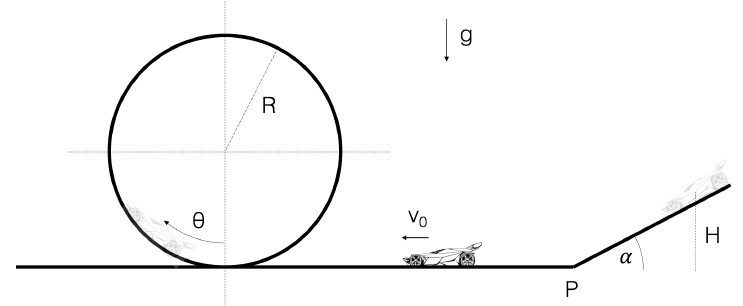
\includegraphics[scale=0.4]{figuras/fig1.jpg}
\caption{Esquema Del problema}
\label{fig:1}
\end{figure}
 \newpage
%%%%%%%%%%%%%%%%%%%%%%%%%%%%%%%%%%%%%%%%%%%%%%%%%%%%%%%%%%%%%%%%%%%%%%%%%%
% Item a 
%%%%%%%%%%%%%%%%%%%%%%%%%%%%%%%%%%%%%%%%%%%%%%%%%%%%%%%%%%%%%%%%%%%%%%%%%%
\section*{Item a}
\addcontentsline{toc}{section}{Item a} 

\begin{figure}[h] 
	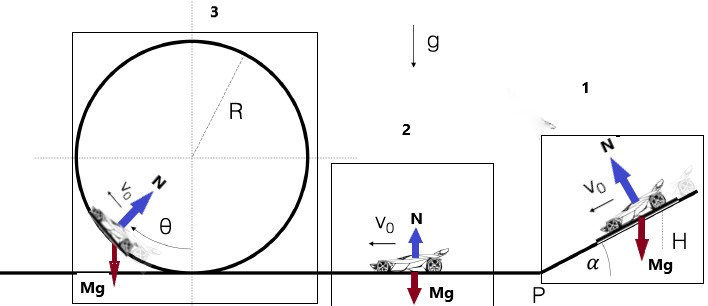
\includegraphics[scale=0.4]{figuras/fig2.jpg}
	\caption{Esquema de las Tres situaciones planteadas}
	\label{fig:2}
\end{figure}

Es conveniente separar el problema en tres situaciones:
\begin{enumerate}
	\item \textbf{El auto cae por un plano inclinado}
	\item \textbf{El auto se mueve a velocidad $v_0$ en linea recta}
	\item \textbf{El auto se mueve en el bucle}
\end{enumerate}

\subsection*{El auto cae por un plano inclinado}
\addcontentsline{toc}{subsection}{El auto cae por un plano inclinado} 

A partir del Diagrama de la \textit{Figura 3}. Se deducen las siguientes
ecuaciones:
\begin{figure}[h] 
	\centering
	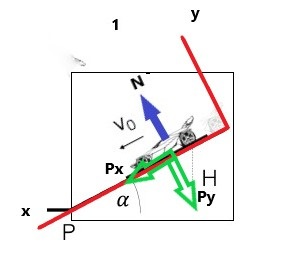
\includegraphics[scale=0.6]{figuras/diag1.jpg}
	\caption{Diagrama de Cuerpo Libre para la Situación (1)}
	\label{fig:3}
\end{figure}
\[\left[ \begin{array}{lll}
 \hat{x}: & P_x = m g \sin{\alpha} = m \ddot{x} & \textbf{(1)}\\
 \hat{y}: &N - P_y = N - m g \cos{\alpha} = m \ddot{y} \overbrace{=}^{\ddot{y}=0} 0 & \textbf{(2)}
\end{array} \right.
\]
Vale aclarar porque la aceleración en $\hat{y}$ es cero y en $\hat{x}$ no. Esto es simplemente porque no hay movimiento en $\hat{y}$ por como esta planeado el eje de coordenadas, luego solo hay movimiento sobre $\hat{x}$.

\subsection*{El auto se mueve a velocidad $v_0$ en linea recta}
\addcontentsline{toc}{subsection}{El auto se mueve a velocidad $v_0$ en linea recta} 

Para la situación (2) podemos plantear el siguiente diagrama:  
\begin{figure}[h] 
	\centering
	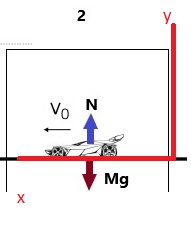
\includegraphics[scale=0.6]{figuras/diag2.jpg}
	\caption{Diagrama de Cuerpo Libre para la Situación (2)}
	\label{fig:4}
\end{figure}
Para este planteamiento, las ecuaciones de Newton nos quedan de la siguiente manera:
\[\left[ \begin{array}{lll}
 \hat{x}: & 0 = m \ddot{x} & \textbf{(3)}\\
 \hat{y}: &N - m g = m \ddot{y} \overbrace{=}^{\ddot{y}=0} 0 & \textbf{(4)}
\end{array} \right.
\]
En este caso, no hay fuerzas externas sobre el auto, (ni rozamiento ni nada que modifique su velocidad). Por lo tanto, el auto ira en movimiento rectilineo uniforme con velocidad $v_0$ cuyo valor coincidira con la velocidad obtenida en el punto $P$. Por otro lado, no hay movimiento en $\hat{y}$, por lo que dicha haceleracion es nula. 

\subsection*{El auto se mueve en el bucle}
\addcontentsline{toc}{subsection}{El auto se mueve en el bucle}

Esta situación es un poco más interesante.

En este caso tenemos al auto entrando en el bucle. El bucle limitara el movimiento del autito dentro de una trayectoria circular. Al ser una trayectoria circular sera conveniente usar coordenadas polares como se indica en la \textit{Figura 5}. 
\begin{figure}[h] 
	\centering
	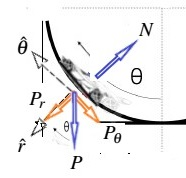
\includegraphics[scale=0.7]{figuras/diag3.jpg}
	\caption{Diagrama de Cuerpo Libre para la Situación (3)}
	\label{fig:5}
\end{figure}

A partír de este diagrama y recordando que las ecuaciones de aceleración y velocidad en polares son:
\[\textbf{v} = \dot{r} \hat{r} + r \dot{\theta} \hat{\theta}\]
\[\textbf{a} = (\ddot{r} - r \dot{\theta}^2)\hat{r} + (r \ddot{\theta} + 2 \dot{r} \dot{\theta})\hat{\theta}\]

Podemos ver que las ecuaciónes de Newton para el Sistema en la situación (3) son:
\[\left[ \begin{array}{lll}
 \hat{r}: &P_r - N =   m g \cos{\theta} - N = m (\ddot{r} - r \dot{\theta}^2) & \\
 \hat{\theta}: &P_{\theta} = - m g \sin{\theta}= m (r \ddot{\theta} + 2 \dot{r} \dot{\theta}) & 
\end{array} \right.
\]
Luego, al ser $R$ constante para el bucle, tenemos que las ecuaciones anteriores se simplifican en las siguientes
\[\left[ \begin{array}{lll}
 \hat{r}: &  m g \cos{\theta} - N = - m R \dot{\theta}^2 & \textbf{(5)}\\
 \hat{\theta}: & - m g \sin{\theta}= m R \ddot{\theta} & \textbf{(6)}
\end{array} \right.
\]
Luego, es notable notar la presencia de aceleración en ambas coordenadas.

Por ultimo, las ecuaciones: $\{(1),(2),(3),(4),(5),(6)\}$ son las ecuaciones de Newton para cada situcación del problema.  

\newpage
%%%%%%%%%%%%%%%%%%%%%%%%%%%%%%%%%%%%%%%%%%%%%%%%%%%%%%%%%%%%%%%%%%%%%%%%%%
% Item b 
%%%%%%%%%%%%%%%%%%%%%%%%%%%%%%%%%%%%%%%%%%%%%%%%%%%%%%%%%%%%%%%%%%%%%%%%%%
\section*{Item b}
\addcontentsline{toc}{section}{Item b}  

Nos piden calcular la fuerza de vinculo, la cual nosotros la llamamos con la letra $N$ (por ser Normal al plano del movimiento) y nos piden calcularla en función de $\theta$, osea $N(\theta)$. 

Podemos obtener esta de dos formas diferentes:
\begin{itemize}
\item[(i) ] Teniendo en cuenta que: $v_0 = R \dot{\theta}$ Por lo que 
$R \dot{\theta}^2 = R \dot{\theta} \dot{\theta}^2 = v_0 \dot{\theta} = \frac{{v_0}^2}{R}$

\item[(ii) ] Teniendo en cuenta que podemos calcular $\dot{\theta}^2$ a partir de la ecuación \textbf{(6)}.
\end{itemize}

---------------------------------------------------------------------

\paragraph{(i)}{
Empecemos calculando $N$ utilizando la ecuación $\frac{{v_0}^2}{R}$ para la aceleración centripeta.

De la ecuación \textbf{(5)}, tenemos que: 

\[ m g \cos{\theta} - N = - m R \dot{\theta}^2 \sii m g \cos{\theta} - N = - m \frac{{v_0}^2}{R} \]


Por lo que se puede despejar muy facilmente una ecuación para la normal, teniendo asi la siguiente ecuación: 
\[ N =  m \left( \frac{{v_0}^2}{R} +  g \cos{\theta} \right) \hspace{0.5cm} \textbf{(7)}\]
}

---------------------------------------------------------------------

Por lo que la fuerza de vinculo puede expresarse utilizando la ecuación \textbf{(7)}. 

Por otro lado, podemos calcular $dot{\theta}$ como sigue en el proximo parrafo.

---------------------------------------------------------------------

\paragraph{(ii)}{ 

Sabemos que: $\ddot{\theta} = \cfrac{d \theta}{dt} = \cfrac{d \dot{\theta}}{d{\theta} } \cfrac{d \theta}{dt} = \dot{\theta} \cfrac{d \dot{\theta}}{d{\theta} }$

Luego, de la ecuación \textbf{(6)}, vemos que:
\[- m g \sin{\theta}= m R \ddot{\theta} = m \dot{\theta} \cfrac{d \dot{\theta}}{d{\theta} }\]
Luego, simplificando las masas y despejando tenemos que:
\[- \frac{g}{R} \int_{0}^{\theta} \sin{\theta} d{\theta} = \int_{0}^{\dot{\theta}} \dot{\theta} d \dot{\theta} \sii -\frac{g}{R} \left[-\cos{\theta} \right]_{0}^{\theta}  = \frac{\dot{{\theta}}^2}{2} \]

Obteniendo asi la siguiente ecuación para $\dot{{\theta}}^2$:
\[ \dot{{\theta}}^2 = - \frac{2g}{R} \left(1- \cos{\theta} \right) \hspace{0.5cm} (8)\]

Luego, como savemos que $v_0 = R \dot{{\theta}}^2$, tenemos que:
\[\frac{{v_0}^2}{R} = (R \dot{{\theta}}^2)^2 \frac{1}{R} = \left(- \frac{2g}{R} (1- \cos{\theta})\right)^2 \frac{1}{R}\]
\[\frac{{v_0}^2}{R} = \frac{4g^2}{R^3} (1-\cos{\theta})^2\]
}

Reemplazando este resultado en la ecuación \textbf{(7)} para la normal, nos queda:
\[N = m \left( g \cos{\theta} +  \frac{4g^2}{R^3} (1-\cos{\theta})^2 \right) \hspace{0.5cm} \textbf{(9)}\]

Luego, las expreciones \textbf{(8)} y \textbf{(9)} son ecuaciónes de la  $N(\theta)$
---------------------------------------------------------------------

%%%%%%%%%%%%%%%%%%%%%%%%%%%%%%%%%%%%%%%%%%%%%%%%%%%%%%%%%%%%%%%%%%%%%%%%%%
% Item c 
%%%%%%%%%%%%%%%%%%%%%%%%%%%%%%%%%%%%%%%%%%%%%%%%%%%%%%%%%%%%%%%%%%%%%%%%%%
\section*{Item c}
\addcontentsline{toc}{section}{Item c} 

Ahora queremos conocer cual debe ser el valor de $v_0$ para que el auto pueda dar la vuelta. 

Obciamente, tenemos un valor minimo y de ahi podremosaumentar este valor sin problemas. 

Dinamicamente, para que el autito pueda dar la vuelta, necesitamos que la fuerza de vinculo no se anule. Si esto pasa, el autito caera (y habra muchos muertos y heridos). 

Entonces, lo que necesitamos es que $N > 0$. En particular, como queremos conocer el valor de $v_0$ que nesecitariamos nos combiene utilizar la ecuación \textbf{(7)} obtenida en el \textit{item b}. 

Planteemos este hecho:

\[ N >0 \sii  m \left( \frac{{v_0}^2}{R} +  g \cos{\theta} \right) > 0 \]
 Como buscamos en particular que la normal no se anule en la parte mas alta, esto seria lo mismo que calcularlo para $\theta = \pi$ por lo que, como $\cos{\pi} = -1$, tenemos que:
 \[\frac{{v_0}^2}{R} -  g   > 0 \sii |v_0|  > \sqrt{Rg}\]
 
Por lo que, el valor minimo para $|v_0|$ es $\sqrt{rg}$.

Si la velocidad es menor, entonces la aceleración centripeta no sera la suficiente y al no haber una aceleración centripeta no puede lograrse el movimiento sobre el bucle.
%%%%%%%%%%%%%%%%%%%%%%%%%%%%%%%%%%%%%%%%%%%%%%%%%%%%%%%%%%%%%%%%%%%%%%%%%%
% Item d 
%%%%%%%%%%%%%%%%%%%%%%%%%%%%%%%%%%%%%%%%%%%%%%%%%%%%%%%%%%%%%%%%%%%%%%%%%%
\section*{Item d}
\addcontentsline{toc}{section}{Item d} 
\def\iangle{35} % Ángulo de giro
\def\arcr{0.7cm} % Radio del arco para marcar ángulos
Para la resolución de este punto, necesitamos hacer una serie de observaciones sobre el movimiento en el plano. 

Nosotros, por como definimos anteriormente el eje de coordenadas para la situacion (1), tenemos que el autito se mueve en dirección $\hat{x}$.
Tomando como $x_0=0$ la posición en x en la cual coincide con el punto más alto del plano inclinado y teniendo en cuenta que llega al piso en el punto $P$ (Ver figura 1 del esquema del problema). Definimos el triangulo rectandulo de la \textit{figura 6} como un modelo del plano inclinado utilizado y asi poder saber cual sera la longitud de la hipotenusa en función de la altura del triangulo (la cual es $H$). 

\begin{figure}[h]
\centering
\begin{tikzpicture}
	\draw (1,1) -- (5,1) -- (5,3) -- cycle;
	%\draw (0,0.5) node{$\theta$}
	\draw[solid =1pt] (1.7,1)
        arc(10 : \iangle : \arcr);
        \node at (4+0.7*\iangle:3.3*\arcr) {$\alpha$};	
	%\draw[thick,black] [shift=(0,0,0) arc (0,1)node[below right]{$\theta$};
	%\draw (1,1) -- (5,1) -- (1,3) -- cycle;
	%\draw (1,1.5) -- (1.5,1.5) -- (1.5,1);

	\node at (3,0.5) {P};
	\node at (3.4,2.7) {X};
	\node at (5.4,1.7) {H};
\end{tikzpicture}
\caption{Triangulo definido para entender la longitud de la hipotenusa en función de la altura}
\end{figure}

Por pitagoras sabemos que: 
\[ X^2 = P^2 + H^2 \]
Necesitamos escribir a $P$ en función de $H$, para poder tener $X(H)$. Sabemos que:
\[\cos{\alpha} = \frac{P}{X} \hspace{0.5cm} \land \hspace{0.5cm} \sin{\alpha} = \frac{H}{X}\]
Luego, como $X=X$, tenemos que:
\[ \frac{P}{\cos{\alpha}} = \frac{H}{\sin{\alpha}} \sii P = \arctan{(\alpha)} H\]
Reemplazando en la ecuación para $X$ planteada para el triangulo, se obtiene que:
\[ X^2 = P^2 + H^2 \sii \rojo{X = H \sqrt{(1+\arctan^2{(\alpha)})}}\]
Como de la ecuación \textbf{(1)} (ver Item a), sabemos que sobre $\hat{x}$ hay un movimiento uniformenente acelerado, cuya aceleración se corresponde con:
\[\ddot{x} = g \sin{(\alpha)}\]
Podemos plantear la siguiente ecuación para $x(t)$ (sabiendo que parte del reposo, es decir $v_0\hat{x} = 0$:
\[H \sqrt{(1+\arctan^2{(\alpha)})} = \frac{1}{2} g \sin{(\alpha)} t^2\]
Esta ecuación involucra al tiempo, pero no involucra a la velocidad, lo cual es lo que nosotros necesitamos, ya que queremos que $\dot{x} = v_0$ en el punto minimo del plano (ya que en el tramo correspondiente a la situación (2) tenemos un MRU). 
Luego, podemos calcular $\dot{x}$ sabiendo que $\ddot{x} = \frac{d \dot{x}}{dt}$ utilizando la ecuación \textbf{(1)}. Si hacemos eso obtenemos:
\[\ddot{x} = \frac{d \dot{x}}{dt} = g \sin{(\alpha)} \sii \int_{0}^{\dot{x}} d \dot{x} =\int_{0}^{t} g \sin{(\alpha)} dt\]
\[\dot{x} = g \sin{(\alpha)} t\]
Luego, $\dot{x} = v_0$ (velocidad al final del plano inclinado). De acá despejamos a $t(v_0)$ para reemplazarlo en la ecuación de la posición del auto sobre el plano.
\[t = \frac{v_0}{g \sin{(\alpha)}}\]
Reemplazamos ahora en la ecuación de movimiento:
\[H \sqrt{(1+\arctan^2{(\alpha)})} = \frac{1}{2} g \sin{(\alpha)} \left( \frac{v_0}{g \sin{(\alpha)}} \right)^2\]
Simplificando:
\[H \sqrt{(1+\arctan^2{(\alpha)})} = \frac{1}{2} \frac{v_0 ^2}{g \sin{(\alpha)}} \]
Despejamos $v_0 ^2$:
\[ 2 H \sqrt{(1+\arctan^2{(\alpha)})} g \sin{(\alpha)} = v_0 ^2\]
\azul{
Agamos un parentesis para ver que es $\sqrt{(1+\arctan^2{(\alpha)})}$:
\[ 1+\arctan^2{(\alpha)} = \frac{\sin^2{\alpha}}{\sin^2{\alpha}} + \frac{\cos^2{\alpha}}{\sin^2{\alpha}} = \frac{1}{\sin^2{\alpha}}\]
Luego, aplicando la raiz:
\[\sqrt{\frac{1}{\sin^2{\alpha}}} = \frac{1}{|\sin{\alpha}|}\]
}
\color{black}
Volviendo a la ecuación de movimiento y volcando este resultado tenemos
\[  \frac{2 H}{|\sin{\alpha}|} g \sin{(\alpha)} = v_0 ^2 \Rightarrow |v_0| = \sqrt{2 H g}\]

Como sabemos que en la situación (2) tenemos un MRU, sabemos que al bucle se va a llegar con la velocidad obtenida arriba. 
Por otro lado, sabemos del \textbf{Item (c)} que $|v_0| > \sqrt{R g}$ para que el auto pueda dar una vuelta al bucle. Por lo tanto, obtenemos la relación:
\[|v_0| > \sqrt{R g} \sii \sqrt{2 H g} > \sqrt{R g} \]
Por lo que la altura minima  debera ser por lo menos:
\[\rojo{H>\frac{R}{2}}\]

%----------------------------------------------------------------------%
%						BIBLIOGRAFIA								   %			
%----------------------------------------------------------------------% 
\phantomsection
\bibliographystyle{unsrt}
\begin{thebibliography}{9}
\bibitem{latexcompanion} 
Juan G. Roederer. 
\textit{Mecanica Elemental}. 
Eudeba, segunda edicion, 2002.

\bibitem{Template} 
Pagina donde se ubica el estilo del template usado,
\\\href{http://www.latextemplates.com/}{\color{B}{Latex Template}}

\bibitem{Codigo Tarea} Codigo de este mismo documento.
\\\href{https://github.com/remusezequiel/Apuntes-Varios-Propios/tree/master/Tarea_2}{\color{B}{Repo Git}}
\end{thebibliography}

\end{document}
